% Copyright 2018-2020 Melvin Eloy Irizarry-Gelpí
\setcounter{chapter}{2}
\chapter{Newton's First Law}
%
In this experiment you will check Newton's first law of motion by considering the effects of diminishing amounts of friction.
%
\section{Preliminary}
%
Newton's \textbf{first law of motion} states that
\begin{itemize}
    \item an object in uniform linear motion will remain in uniform linear motion unless acted by an external (net) force.
\end{itemize}
\textbf{Uniform linear motion} is motion where the \textbf{velocity is constant}. Recall that velocity is a vector physical quantity: velocity has a \textbf{magnitude} (speed) and a \textbf{direction}. If an object moves with constant velocity, then both the magnitude and the direction are fixed in time. If there is an external net force acting on the object, then the velocity will change with time due to this force, and the motion will not be uniform linear motion.

If velocity is constant, then it is not changing with time. Thus, when velocity is constant, the rate of change of velocity with time is zero. But acceleration is defined as the rate of change of velocity with time. Thus, an object in uniform linear motion will have zero acceleration.

Friction is an ubiquitous force. It is almost always present in most motions. There are many kinds of frictional forces, but the most relevant one for this experiment is \textbf{kinetic friction}. The most important aspect of kinetic friction is that it is approximately constant in magnitude, and directly proportional to the amount of normal force on the surface. Later you will learn that a \textbf{constant net force} leads to a \textbf{constant acceleration}. You have done two experiments with constant acceleration: the free-falling picket fence and the cart moving along an incline. In both of this you learned that the value of the constant acceleration can be learned from the slope of the velocity versus time chart.
%
\section{Experiment}
%
You use a motion sensor to measure the position, velocity, and acceleration of a cart. The cart has a mechanism that allows kinetic friction to be adjusted. You consider motions along a track with increasing amounts of kinetic friction, and extrapolate your results to verify that Newton's first law of motion is indeed correct.
%
\section{Analysis}
%
For this experiment you are only going to analyze the velocity and time data. Here are some steps to follow for each run:
\begin{enumerate}
    \item Make a scatter chart with velocity in the vertical axis and time in the horizontal axis.
    \item Restrict to the region where the shape is appropriately linear. This might involve deleting data from the beginning and/or the end.
    \item Once the linear segment is the only part remaining, add a best-fit line and record the value of the intercept and the slope.
\end{enumerate}
%
\section{My Data}
%
My data consist of eight runs. For run 1 the friction pad was retracted all the way. For runs 2, 3, and 4 the friction pad was brought closer to the track, but the effect was not noticeable on the slope. Starting with run 5, you see the effects of the friction pad change the value of the slope. Run 8 is when the friction pad is at its lowest configuration.
%
\section{Your Data}
%
You should have about 6 runs of data with the friction pad close to the track, and one run with the friction pad not touching the track.
%
\newpage
\section{Your Laboratory Report}
%
Your laboratory report should include the following:
\begin{enumerate}
    \item A table like Table \ref{table:03.results} with your results for the slope and intercept of the velocity versus time charts.
    \item A scatter chart like Figure \ref{figure:03.run-1} with velocity in the vertical axis and time in the horizontal axis, for your run where the friction pad was not touching the track. Include the whole run.
    \item A scatter chart like Figure \ref{figure:03.run-8} with velocity in the vertical axis and time in the horizontal axis, for your run where the friction pad was at its lowest. Show the whole run and label in the chart when the cart is being accelerated by the spring, when the cart is moving along the track, and when the cart is stopped.
\end{enumerate}
You should also answer the following questions:
\begin{enumerate}
    \item If there is no friction between the cart and the track, what should be the value of the slope in the velocity versus time chart?
    \item What happens to the value of the slope as the amount of friction is reduced?
    \item Can you extrapolate your observations and confirm or dismiss Newton's first law of motion?
    \item What is the physical meaning of the intercept? Should all intercept values be very different?
    \item How can you use the values of the intercept to judge the quality of reproducing the same initial conditions?
\end{enumerate}
%
\newpage
\section{Tables}
%
\vspace{\stretch{1}}
\begin{table}[ht]
    \centering
    \begin{tabular}{|l|r|r|}
        \hline
        Run & Slope (m/s$^{2}$) & Intercept (m/s) \\
        \hline
        1 & \textminus 0.050 & 0.283 \\
        2 & \textminus 0.049 & 0.298 \\
        3 & \textminus 0.051 & 0.291 \\
        4 & \textminus 0.052 & 0.287 \\
        5 & \textminus 0.058 & 0.311 \\
        6 & \textminus 0.091 & 0.293 \\
        7 & \textminus 0.131 & 0.268 \\
        8 & \textminus 0.194 & 0.339 \\
        \hline
    \end{tabular}
    \caption{Slope and Intercept values for the velocity versus time charts.}
    \label{table:03.results}
\end{table}
\vspace{\stretch{1}}
%
\FloatBarrier
\newpage
\section{Figures}
%
\vspace{\stretch{1}}
\begin{figure}[ht]
    \centering
    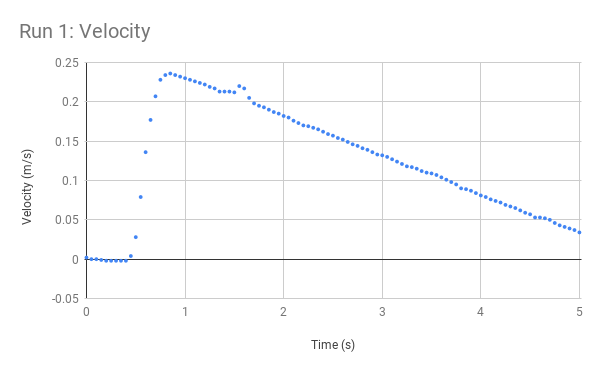
\includegraphics[scale=0.71]{image/03-first-law/Run-1-Velocity.png}
    \caption{Run 1: No friction pad}
    \label{figure:03.run-1}
\end{figure}
\vspace{\stretch{1}}
%
\begin{figure}[ht]
    \centering
    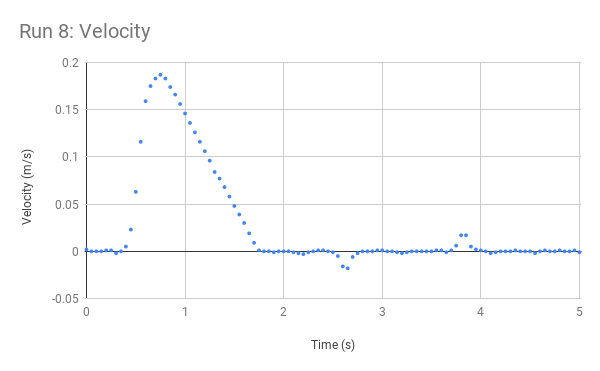
\includegraphics[scale=0.71]{image/03-first-law/Run-8-Velocity.png}
    \caption{Run 8: Friction pad at its lowest}
    \label{figure:03.run-8}
\end{figure}
%